% !Mode:: "TeX:UTF-8"

%Composed by Y.B. TANG (ybtang21c@gmail.com), spring-2011
%tex distribution: Texlive / MikTex 2010
%recommended editer: Eclipse + Texlipse
%usage: compile with XeLatex

%option: red, brown, blue
% \documentclass[14pt,mathserif]{beamer}
% \documentclass[14pt]{beamer}
\documentclass[usepdftitle=false, 14pt]{beamer}

\usepackage{amsmath,amsfonts,amssymb,amsthm,bm}
% \usepackage{txfonts} %another style of math fonts
\usepackage{beamerthemesplit,color,graphics}
\usepackage{ulem} %erase line
\usepackage{esint} %any type of integral symbol
% \usepackage{yhmath} %圆弧帽:\wideparen{AB}

\usepackage{bbding}%各种五角星
% \FiveStar,\FiveStarOpen,\FiveStarLines,\FiveStarShadow
% \FiveStarOutline,\FiveStarCenterOpen,\FiveStarOpenDotted
% \FiveStarConvex,\FiveStarOutlineHeavy,\FiveStarOpenCircled

%==============XeCJK==============================
\usepackage[slantfont,boldfont,CJKchecksingle]{xeCJK}
\setmainfont{Times New Roman}
\setCJKmainfont[BoldFont={Adobe Heiti Std},
	ItalicFont={Adobe Kaiti Std},
    SlantedFont={Adobe Song Std},
%     BoldItalicFont={Weibei SC},
     BoldSlantedFont={Adobe Fangsong Std}
	]{Adobe Heiti Std}
\punctstyle{CCT}
\usepackage{xeCJKfntef}%汉字加点和可断行的下划线
% 
% \newCJKfontfamily[Wawa]\Wawati{Wawati SC}
% \newCJKfontfamily[STLi]\stliti{STLiti}

\usefonttheme{professionalfonts}

\newcommand{\fs}[1]{\fontspec{#1}\CJKfontspec{#1}}

%

% %==============std fontspec settings==============
% \usepackage[no-math,cm-default]{fontspec}
% % \newfontfamily\zhfont[BoldFont=Adobe Heiti Std]{Adobe Heiti Std}
% \newfontfamily\zhfont[BoldFont=Adobe Heiti Std]{Adobe Kaiti Std}
% % 
% % %==============spacing of CH in Xetex==============
% \usepackage{zhspacing}
% \zhspacing

%==============layout setting==============
\setlength{\parindent}{0pt}  

%==============beamer configuration==============
\setbeamertemplate{theorems}[normal font]

%============beamer theme setting #2============
\mode<presentation>{
	\usetheme{Copenhagen} %Copenhagen, Warsaw, CambridgeUS
  	\usecolortheme{lily} %rose, seahorse, lily, crane
  	\usefonttheme{serif}
  	\usefonttheme{structurebold}
  	\useoutertheme{infolines}
%   \beamertemplateshadingbackground{brown!5}{yellow!10}
% 	\setbeamercolor{frametitle}{bg=white}	
%  	\setbeamercovered{transparent}
}

%============TOC setting============
% \AtBeginSection{
%    \begin{frame}{内容提要}
%      \tableofcontents[currentsection,hideallsubsections]
%    \end{frame}
% }
% \AtBeginSubsection{
%    \begin{frame}{内容提要}
%      \tableofcontents[currentsection,currentsubsection]
%    \end{frame}
% }
% \AtBeginSection{
%   \frame{\tableofcontents[sections={\thesection}]}
% }

%===============macros====================
\newcommand{\bb}{\bf\color{blue}}
\newcommand{\ba}[1]{\alert{\bf #1}}
\newcommand*{\e}{\ensuremath{\varepsilon}}
\renewcommand{\b}{\color{blue}}
\newcommand*{\p}{\ensuremath{\partial}}
\newcommand{\limn}{\ensuremath{\lim\limits_{n\to\infty}}}
\newcommand{\sumn}{\ensuremath{\sum\limits_{n=1}^{\infty}}}
\newcommand*{\df}[2]{\displaystyle\frac{\,{#1}\,}{\,{#2}\,}}
\newcommand*{\limx}[1]{\ensuremath{\lim\limits_{x\to{#1}}}}
\newcommand*{\limdx}{\ensuremath{\lim\limits_{\Delta x\to 0}}}
\newcommand*{\dx}{\Delta x}
\newcommand{\dint}{\ensuremath{\displaystyle\int}}
\renewcommand{\d}{\mathrm{d}}
\newcommand{\ds}{\displaystyle}

%================exampleblock counter===================
% \newcounter{examplecounter}
% \usecounter{examplecounter}
% \setcounter{examplecounter}{1}
% \newcommand{\exno}{{\bf
% 例\arabic{examplecounter}}\refstepcounter{examplecounter}}

%================block setting test=====================
% \definecolor{beamer@blendedred}{rgb}{0.7,0.2,0.2} % use structure theme to change
% \definecolor{beamer@blendedblue}{rgb}{0.2,0.2,0.7} % use structure theme to change
% \definecolor{beamer@blendedyellow}{rgb}{0.7,0.7,0.2}

% \setbeamercolor{structure}{fg=beamer@blendedred}

% \setbeamercolor{block title}
% {use=structure,fg=structure.fg,bg=structure.fg!20!bg}
% \setbeamercolor{block title alerted}
% {use=alerted text,fg=alerted text.fg,bg=alerted text.fg!20!bg}
% \setbeamercolor{block title example}
% {use=example text,fg=example text.fg,bg=example text.fg!20!bg}

% \setbeamercolor{block body}
% {parent=normal text,use=block title,bg=block title.bg!50!bg}
% \setbeamercolor{block body alerted}
% {parent=normal text,use=block title alerted,bg=block title alerted.bg!50!bg}
% \setbeamercolor{block body example}
% {parent=normal text,use=block title example,bg=block title example.bg!50!bg}

% \setbeamercolor{titlelike}{parent=structure,bg=white!90!red}
%=======================================================

%===============title setting====================

\title{Advanced Mathematics II}
\author[NUDT]{唐扬斌\\
\texttt{\small ybtang21c@gmail.com\\tangyangbin@gfkd.mtn\\CP: 18374857376}}
\institute[NUDT]{National University of Defense Technology}
\date[Spring 2016]{Spring 2016}

%===============document begins here==============

\begin{document}

%L-1.tex:2010秋季学期考试讲评
%L01.tex:常微分方程的概念与一阶微分方程的解法
%L04-Ch07-1orderDE-HW:一阶微分方程求解的课堂思考题
%L02.tex:二阶微分方程的解法
%L03_ch7ex1.tex:常微分方程习题课
%L04.tex:向量运算与空间直线、平面的方程
%L05.tex:空间平面与直线
%L05-Ch08-ex1.tex
%L06.tex:空间曲面
%L07.tex:空间曲线
%L08_ch8ex2.tex:空间曲面与曲线习题课
%L09.tex:向量值函数
%L10.tex:多元函数极限、连续与偏导数
%L11.tex:全微分与复合函数求导
%L12.tex:多元复合函数与隐函数的偏导数
%L13_ch9ex1:多元函数的偏导数习题课
%L14.tex:方向导数与梯度、Hessian矩阵及Taylor公式
%L15.tex:多元函数的极值与条件极值
%L16_ch10ex2.tex:多元函数微分的应用
%L16_ch10ex3.tex:多元函数微分学及其应用(All)
%L17.tex:重积分的概念与性质
%L18.tex:重积分的计算
%L19.tex:坐标变换与重积分的计算
%L20.tex:重积分的应用
%L21.tex:重积分习题课
%L22.tex:曲线积分
%L23.tex:Green公式与保守场
%L24.tex:曲面积分
%L25.tex:Gauss公式与Stokes公式
%L26_ch12ex.tex:曲线与曲面积分习题课
% L26_ch12ex-1.tex:曲线与曲面积分习题课,2016春
%L27_ch12ex.tex:对称性在积分计算中的应用
%L28.tex:幂级数及其应用
%L29.tex:Fourier级数
%L30.tex:《高等数学(下)》复习

%fontTest.tex:各种字体的演示

%    % !Mode:: "TeX:UTF-8"

\begin{frame}{第二十一讲、重积分的计算习题课}
	\linespread{1.5}
	\begin{enumerate}
	  \item {\bf 内容与要求}%{\b (\S 11.4)}
	  \begin{itemize}
		\item 重积分的概念与性质
		\item 重积分的计算
		\item 坐标变换下的重积分
	    \item 重积分的应用
	  \vspace{1em}
	  \end{itemize}
% 	  \item {\bf  课后作业:}
% 	  \begin{itemize}
% 	    \item {\b 习题11.4:1,4,6(2),9,12}
% 	  \end{itemize}
	\end{enumerate}
\end{frame}

\begin{frame}{二重积分的计算}
	\linespread{1.5}\pause 
	\begin{exampleblock}{{\bf 例1:}计算下列二重积分\hfill}\pause 
		\begin{enumerate}
		  \item $\ds\iint_Dxye^{xy^2}\d\sigma,\,D=\{0\leq x\leq 1,0\leq
		  y\leq 1\}$\pause 
		  \item $\ds\iint_D\df 1{x+y}\d\sigma,\,D=\{0\leq x\leq 1,1\leq x+y\leq
		  2\}$\pause 
		  \item $\ds\iint_D|x^2+y^2-4|\d\sigma,\,D=\{x^2+y^2\leq 9\}$\pause 
		  \item $\ds\iint_D(x+y)\mathrm{sgn}(x-y)\d\sigma,\,D=\{0\leq x\leq 1,0\leq
		  y\leq 1\}$
		\end{enumerate}
	\end{exampleblock}
\end{frame}

\begin{frame}{二重积分的积分次序}
	\linespread{1.2}\pause 
	\begin{exampleblock}{{\bf 例2:}改变下列累次积分的次序\hfill}\pause 
		\begin{enumerate}
		  \item $\dint_0^1\dint_0^xf(x,y)\d
		  y\d x+\dint_1^2\dint_0^{2-x}f(x,y)\d y\d x$\pause
		  \item $\dint_0^{2a}\dint_{\sqrt{2ax-x^2}}^{\sqrt{2ax}}
		  f(x,y)\d y\d x,\;(a>0)$\pause 
		  \item $\dint_0^{2\pi}\dint_0^{\sin x}f(x,y)\d y\d x$
		\end{enumerate}
	\end{exampleblock}
\end{frame}

\begin{frame}{二重积分与定积分}
	\linespread{1.2}\pause 
	\begin{exampleblock}{{\bf 例3}\hfill}
		设$f(x)$在区间$[a,b]$连续且恒大于零,证明:
		$$\dint_a^bf(x)\d x\dint_a^b\df{\d x}{f(x)}\geq (b-a)^2$$
	\end{exampleblock}
	\bigskip\pause 
	\begin{exampleblock}{{\bf 例3'}\hfill}
		利用二重积分的方法证明
		$$\left[\dint_a^bf(x)g(x)\d x\right]^2\leq
		\dint_a^bf\,^2(x)\d x\dint_a^bg^2(x)\d x$$
	\end{exampleblock}
\end{frame}

\begin{frame}{二重积分与坐标变换}
	\linespread{1.2}\pause 
	\begin{exampleblock}{{\bf 例4}\hfill}
		计算
		$$\iint_{x^2+y^2\leq 1}\df{\d\sigma}{(x^2+y^2)^m}$$
	\end{exampleblock}\pause 
	\begin{exampleblock}{{\bf 例5}\hfill}
		设$f(x)$可微,$f(0)=0,\,f\,'(0)=1$,求
		$$\lim\limits_{t\to 0^+}\df 1{\pi t^3}
		\iint_{x^2+y^2\leq t^2}f\left(
		\sqrt{x^2+y^2}\right)\d x\d y$$
	\end{exampleblock}
\end{frame}

\begin{frame}{二重积分与坐标变换}
	\linespread{1.2}
	\begin{exampleblock}{{\bf 例6}\hfill}
		计算
		$$\iint_{x^2+4y^2\leq 1}(x^2+y^2)\d\sigma$$
	\end{exampleblock}
	\pause
	\alert{设$x=x(u,v),y=y(u,v)$,\pause 则}
	$$\alert{\iint_Df(x,y)dxdy=\iint_D
	f(x,y)\left|\df{\p(x,y)}{\p(u,v)}\right|
	\d u\d v}$$
\end{frame}

\begin{frame}{二重积分与坐标变换$^*$}
	\linespread{1.2}\pause 
	\begin{exampleblock}{{\bf 例7}}
		通过适当的变量替换,将下列二重积分化为定积分\pause 
		\begin{enumerate}
		  \item $\ds\iint_{|x|+|y|\leq 1}f(x+y)\d\sigma$\pause 
		  \item $\ds\iint_Df(xy)\d\sigma$,$D$由$xy=1,xy=2,y=x$,
		  
		  $y=4x,(x>0,y>0)$围成\pause 
		  \item $\ds\iint_{x^2+y^2\leq 1} f(ax+by+c)\d\sigma,\;(a^2+b^2\ne 0)$
		\end{enumerate}
	\end{exampleblock}
\end{frame}

\begin{frame}{三重积分的计算}
	\linespread{1.2} 
	\begin{exampleblock}{{\bf 例8}\hfill}
		设$f(z)$连续,证明:
		$$\iiint_{x^2+y^2+z^2\leq 1}f(z)\d V=\pi\dint_{-1}^1f(u)(1-u^2)\d u$$
	\end{exampleblock}
	\bigskip\pause
	\begin{exampleblock}{{\bf 例9}\hfill}
		计算三重积分
		$$\iiint_{\Omega}z^2\d V,\;\Omega:x^2+y^2+z^2\leq 1,\,z\geq 0$$
	\end{exampleblock}	
\end{frame}

\begin{frame}{三重积分的积分次序}
	\linespread{1.2}
	\begin{columns}
		\column{.6\textwidth}
			\begin{exampleblock}{{\bf 例10}\hfill}
				按给定的积分次序重写累次积分
				$$\dint_0^1\dint_0^x\dint_0^{xy}f(x,y,z)\d z\d y\d x$$
				\begin{enumerate}
				  \item 先$y$后$z$后$x$
				  \item 先$x$后$z$后$y$
				\end{enumerate}
			\end{exampleblock}
		\column{.4\textwidth}
			\begin{center}
				\pause \resizebox{!}{5cm}{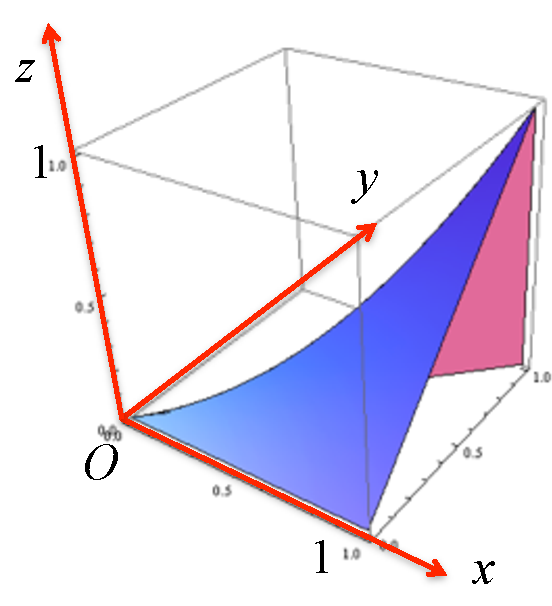
\includegraphics{./images/ch11/xyzC.pdf}}
			\end{center}
	\end{columns}
\end{frame}

\begin{frame}{三重积分与坐标变换}
	\linespread{1.5}\pause
	\begin{exampleblock}{{\bf 例11}\hfill}
		针对给定的积分区域,分别用柱坐标和球坐标将三重积分$\ds\iiint_{\Omega}
		f(x,y,z)\d V$化为累次积分:\pause
		\begin{enumerate}
		  \item $\Omega:\,z\leq\sqrt{4-x^2-y^2},\,3z\geq x^2+y^2$\pause 
		  \item $\Omega:\, z\geq x^2+y^2,\,z\leq x$
		\end{enumerate}
	\end{exampleblock}
\end{frame}

\begin{frame}{三重积分与坐标变换}
	\linespread{1.2}
	\begin{exampleblock}{{\bf 例12}\hfill}
		将三重积分
		$$\dint_0^1\dint_{-\sqrt{y-y^2}}^{\sqrt{y-y^2}}
		\dint_0^{\sqrt{3(x^2+3y^2)}}f\left(
		\sqrt{x^2+y^2+z^2}\right)\d z\d x\d y$$
		分别化为柱坐标和球坐标下的三重积分。
	\end{exampleblock}
\end{frame}

\begin{frame}{三重积分与坐标变换}
	\linespread{1.2}
	\begin{exampleblock}{{\bf 例13}\hfill}
		计算积分
		$$\iiint_{\Omega}(x+y+z)^2\d V,$$
		其中$\Omega:\;\df{x^2}{a^2}+\df{y^2}{b^2}+\df{z^2}{c^2}\leq 1$
	\end{exampleblock}
% 	{\bf 注:}令
% 	$$x=ar\sin\varphi\cos\theta,\,y=br\sin\varphi\sin\theta,\,z=cr\cos\varphi$$
% 	则
% 	$$\alert{\iiint_{\Omega}fdV=abc\iiint_{\Omega}fr^2\sin\varphi drd\varphi
% 	d\theta}$$
\end{frame}

\begin{frame}{三重积分与坐标变换}
	\linespread{1.2}
	\begin{exampleblock}{{\bf 例14}\hfill}
		计算由以下平面所围成的立体体积:
		$$a_ix+b_iy+c_iz=\pm h_i,\;i=1,2,3,$$
		其中:$a_i,b_i,c_i(i=1,2,3)$为常数,且
		$$\Delta=\left|\begin{array}{ccc}
		a_1 & b_1 & c_1\\ a_2 & b_2 & c_2 \\ a_3 & b_3 & c_3
		\end{array}\right|\ne 0$$
	\end{exampleblock}
\end{frame}

% \begin{frame}{三重积分与坐标变换*}
% 	\linespread{1.2}
% 	\begin{exampleblock}{{\bf 例15}\hfill}
% 		求以下曲面在第一卦限中所围立体体积
% 		$$\left(\df xa+\df yb\right)^2+\left(\df zc\right)^2=1,$$
% 		其中$a,b,c>0$。
% 	\end{exampleblock}
% \end{frame}

\begin{frame}{三重积分的计算*}
	\linespread{1.2}
	\begin{exampleblock}{{\bf 例15}\hfill}
		计算极限
		$$\lim\limits_{n\to\infty}\df 1{n^4}\iiint_{r\leq n}[r]\d V,$$
		其中$r=\sqrt{x^2+y^2+z^2}$。
	\end{exampleblock}
	\pause
	$$\alert{\df 43\pi\left[n^4-\sum
	\limits_{k=1}^nk^3\right]}$$
\end{frame}

\begin{frame}{三重积分的计算*}
	\linespread{1.2}
	\begin{exampleblock}{{\bf 例16}\hfill}
		设$f(x)$可微,
		$$F(t)=\iiint_{x^2+y^2+z^2\leq t^2}f(x^2+y^2+z^2)\d V,$$
		求$F\,'(t)$。
	\end{exampleblock}
\end{frame}

\begin{frame}{三重积分的计算*}
	\linespread{1.2}
	\begin{exampleblock}{{\bf 例17}\hfill}
		设$f(x)$可微,
		$$F(x)=\dint_0^x\d v\dint_0^v\d u\dint_0^uf(t)\d t,$$
		求$F\,'(x)$。
	\end{exampleblock}
% 	\pause
% 	$$\alert{\df{x^2}2\dint_0^xf(t)dt-x\dint_0^xtf(t)dt
% 	+\df 12\dint_0^xt^2f(t)dt}$$
\end{frame}

% \begin{frame}{三重积分的计算*}
% 	\linespread{1.2}
% 	\begin{exampleblock}{{\bf 例19}\hfill}
% 		$$I=\iiint_{x^2+y^2+z^2}(x+y+z-10)\d V,$$
% 		证明:
% 		$$28\sqrt 3\pi\leq I\leq 52\sqrt 3\pi$$
% 	\end{exampleblock}
% % 	\pause
% % 	$$\alert{\df{x^2}2\dint_0^xf(t)dt-x\dint_0^xtf(t)dt
% % 	+\df 12\dint_0^xt^2f(t)dt}$$
% \end{frame}

\begin{frame}{重积分的应用}
	\linespread{1.2}
	\begin{exampleblock}{{\bf 例18}\hfill}
		在一半径为$R$的球内,以某条直径为轴打一个半径为$r(r<R)$的
		圆孔,求打孔后球内剩余部分的体积。
	\end{exampleblock}
	\bigskip\pause
	\begin{exampleblock}{{\bf 例19}\hfill}
		求锥面$3(x^2+y^2)=(z-3)^2$与$z=0$所围的内切球面
		与该锥面所围成的立体的体积。
	\end{exampleblock}
\end{frame}

% \begin{frame}{重积分的应用}
% 	\linespread{1.2}
% 	\begin{exampleblock}{{\bf 例22}\hfill}
% 		某火山的表面为曲面
% 		$$z=h\,\mathrm{exp}\left(-\df{\sqrt{x^2+y^2}}{4h}\right),$$
% 		其中$h>0,\,x^2+y^2\leq R^2$。经历一次喷发后,共在火山上落下体积为
% 		$V$的一层等厚度的熔岩,求落下的熔岩厚度。
% 	\end{exampleblock}
% \end{frame}

\begin{frame}{$n$重积分*}
	\linespread{1.2}
	\begin{exampleblock}{{\bf 例20}\hfill}
		求$n$维单纯形
		$$T_n:\; x_i\geq 0\,(i=1,2,\ldots,n),\;
		\sum\limits_{i=1}^nx_i\leq a$$
		的体积$(a>0)$。
	\end{exampleblock}
	\pause
	$$\alert{\df{a^n}{n!}}$$
\end{frame}

\begin{frame}{$n$重积分*}
	\linespread{1.2}
	\begin{exampleblock}{{\bf 例21}\hfill}
		证明:
		$$\dint_0^t\d t_1\dint_0^{t_1}\d t_2\ldots
		\dint_0^{t_{n-1}}\prod\limits_{i=1}^nf(t_i)\d t_n
		=\df 1{n!}\left[\dint_0^tf(s)\d s\right]^n$$
	\end{exampleblock}
\end{frame}

\begin{frame}{$n$重积分*}
	\linespread{1.2}
	\begin{exampleblock}{{\bf 例22}\hfill}
		求$n$维单位球
		$$\sum\limits_{k=1}^nx_k^2\leq 1$$
		的体积。
	\end{exampleblock}
	\pause
	$$\alert{\Gamma(\alpha)=\dint_0^{+\infty}x^{\alpha-1}e^{-x}dx,\;(\alpha>0)}$$
	\pause
	$$\alert{V_n=\df{2\pi^{n/2}}{n\Gamma(n/2)}}$$
\end{frame}

\begin{frame}
	\linespread{1.2}
	\begin{exampleblock}{{\bf 课后练习1}\hfill}
		设$f(x)$在$[a,b]$上单调递增且恒为正,证明
		$${\dint_0^1xf\,^2(x)\d x}{\dint_0^1f(x)\d x}\leq
		{\dint_0^1f\,^2(x)\d x}{\dint_0^1xf(x)\d x}$$
	\end{exampleblock}
	\bigskip
	\begin{exampleblock}{{\bf 课后练习2}\hfill}
		设$a^2+b^2=1,\, D:x^2+y^2\leq 1$,证明
		$$\iint_Df(ax+by)\d x\d y=2\dint_{-1}^1f(u)\sqrt{1-u^2}\d u.$$
	\end{exampleblock}
\end{frame}

\begin{frame}{三重积分与坐标变换*}
	\linespread{1.2}
	\begin{exampleblock}{{\bf 例23}\hfill}
		求以下曲面在第一卦限中所围立体体积
		$$\left(\df xa+\df yb\right)^2+\left(\df zc\right)^2=1,$$
		其中$a,b,c>0$。
	\end{exampleblock}
\end{frame}

%=====================================

% \begin{frame}{title}
% 	\linespread{1.2}
% 	\begin{exampleblock}{{\bf title}\hfill}
% 		123
% 	\end{exampleblock}
% \end{frame}
% 
% \begin{frame}{title}
% 	\linespread{1.2}
% 	\begin{block}{{\bf title}\hfill}
% 		123
% 	\end{block}
% \end{frame}
   \begin{frame}{曲线积分与曲面积分}
	\linespread{1.2}
	\begin{enumerate}
	  \item 曲线和曲面积分的计算
	  \begin{itemize}
	    \item {\it 第一型:方向无关,第二型:方向敏感}
	    \item {\it 第一型:质量类应用;第二型:向量场类应用}
	  \end{itemize}
	  \item Green公式和Gauss公式
	  {\it
	  \begin{itemize}
	    \item Green公式的证明
	    \item “补全”和“挖洞”
	    \item 全微分与原函数(势函数)
	    \item 散度、旋度、无源场、无旋场、保守场、C-R条件
	  \end{itemize}
	  }
	  \item 对称性在各种积分中的应用
	  \item 不同类型积分之间的相互转换
	\end{enumerate}
\end{frame}

\begin{frame}
	\linespread{1.5}
% 	$\star$
	\ba{1、}设$L$为曲线$x=\df{3at}{1+t^3},y=\df{3at^2}{1+t^3}$上$t$由
	$0$到$+\infty$的一段,$a>0$,则$\dint_Lx\d y-y\d x=$
	\underline{\uncover<2->{\;\b{$3a^2$}}\;}.\\[1em]
	
% 	\pause\pause
	\ba{2、}$f(x)$连续可导,$L$为$(3,2/3)$到$(1,2)$的直线,
	则$\dint_L\df{1+y^2f(xy)}y\d x+\df x{y^2}[y^2f(xy)-1]\d y=$
	\underline{\uncover<3->{\;\b{$-4$}}\;}.\\[1em]
	
% 	\pause\pause
	\ba{3、}$\ds\iint_{z=\sqrt{a^2-x^2-y^2}}(x+y+z)\d S=$
	\underline{\uncover<4->{\;\b{$\pi a^3$}}\;}.\\[1em]
\end{frame}

\begin{frame}
	\linespread{1.5}
% 	$\star$
	\ba{4、}设$\Sigma$为平面$x+y+z=1$在第一卦限的上侧,$f(x,y,z)$连续,则
	$\ds\iint_{\Sigma}[f(x,y,z)+x]\d y\d z-[2f(x,y,z)-y]\d z\d x+
	[f(x,y,z)+z]\d x\d y=$
	\underline{\uncover<2->{\;\b{$\df12$}}\;}.\\[1em]
	
% 	\pause\pause
	\ba{5、}设$\Sigma$为锥面$z=\sqrt{x^2+y^2}(0\leq z\leq 1)$的下侧,则
	$\ds\iint_{\Sigma}x\d y\d z+2y\d z\d x+3(z-1)\d x\d y=$
	\underline{\uncover<3->{\;\b{$2\pi$}}\;}.\\[1em]
	
% 	\pause\pause
	\ba{6、}设$L$是摆线$x=t-\sin t-\pi,y=1-\cos t$从$t=0$
	到$t=2\pi$的一段,则$\dint_L\df{(x-y)\d x+(x+y)\d y}{x^2+y^2}=$
	\underline{\uncover<4->{\;\b{$\pi$}}\;}.\\[1em]
\end{frame}

\begin{frame}
	\linespread{1.5}
	\ba{例:}设$L_1:\df{x^2}{4}+\df{y^2}{9}=1,L_2:
	\df{x^2}{9}+\df{y^2}{4}=1$,
	二者所围封闭区域分别为$D_1,D_2$,则下列正确的是
	(\underline{\uncover<2->{\;\b{C}}\;})
	\begin{enumerate}[(A)]
	  \item $\dint_{L_1}(x+y^2)\d s=2\dint_{L_2}y^2\d s$
	  \item $\dint_{L_1}(x^2+y)\d s=2\dint_{L_2}(x^2+y)\d s$
	  \item $\ds\iint_{D_1}(x+y^3)\d\sigma=2\ds\iint_{D_2}(x+y^3)\d\sigma$
	  \item $\ds\iint_{D_1}(x^2+y)\d\sigma=2\ds\iint_{D_2}(x^2+y)\d\sigma$
	\end{enumerate}
\end{frame}

\begin{frame}
	\linespread{1.5}
	\ba{例:}$f(x,y)$偏导连续,曲线$L:f(x,y)=1$过第二象限的点$M$
	  和第四象限的点$N$,$\Gamma$为$L$上从$M$到$N$的一段弧,则下列
	  小于零的是
	(\underline{\uncover<2->{\;\b{B}}\;})
	\begin{enumerate}[(A)]
	  \item $\dint_{\Gamma}f(x,y)\d x$
	  \item $\dint_{\Gamma}f(x,y)\d y$
	  \item $\ds\int_{\Gamma}f(x,y)\d s$
	  \item $\ds\int_{\Gamma}f\,'_x(x,y)\d x+f\,'_y(x,y)\d y$
	\end{enumerate}
\end{frame}

\begin{frame}
	\linespread{1.5}
	\ba{例:}设曲面$S_1:x^2+y^2+z^2=1(z\geq
	  0)$,$S_2$为$S_1$在第一卦限中的部分,
	  则以下正确的是
	(\underline{\uncover<2->{\;\b{C}}\;})
	\begin{enumerate}[(A)]
	  \item $\ds\iint_{S_1}x\d S=4\iint_{S_2}x\d S$
	  \item $\ds\iint_{S_1}y\d S=4\iint_{S_2}x\d S$
	  \item $\ds\iint_{S_1}z\d S=4\iint_{S_2}x\d S$
	  \item $\ds\iint_{S_1}xyz\d S=4\iint_{S_2}xyz\d S$
	\end{enumerate}
\end{frame}

\begin{frame}
	\linespread{1.5}
	\ba{例:}设$f(r)$二阶连续可微,$r=\sqrt{x^2+y^2+z^2}$,
  	若$\mathrm{div}(\bigtriangledown\,f(r))=0$,则$f(r)=$
	(\underline{\uncover<2->{\;\b{B}}\;})
	\begin{enumerate}[(A)]
	  \item $C_1r+C_2$
      \item $C_1/r+C_2$
      \item $C_1r^2+C_2$
      \item $C_1/r^2+C_2$
	\end{enumerate}
\end{frame}

\begin{frame}
	\linespread{1.2}
	\alert{提示:}{\it\b 几个建议单独记忆的公式 
	\begin{enumerate}[(1)]
	  \item \b$\mathrm{div}(\bm{v})=\bigtriangledown\cdot\bm{v}$
	  \item \b$\mathrm{rot}(\bm{v})=\bigtriangledown\times\bm{v}$
	  \item \b$\mathrm{div}(u\;\bm{v})=u\;\mathrm{div}\bm{v}
	  +\bm{v}\cdot\bigtriangledown u$
	  \item \b$\mathrm{rot}(u\;\bm{v})=u\;\mathrm{rot}\bm{v}
	  +\bm{v}\times\bigtriangledown u$
	  \item \b$\mathrm{div}(\bigtriangledown r)=\df2r$,
	  \hspace{1cm} $(r=\sqrt{x^2+y^2+z^2})$
	  \item \b$\mathrm{rot}(\bigtriangledown r)=0$,
	  \hspace{1cm} $(r=\sqrt{x^2+y^2+z^2})$
	\end{enumerate}
	}
\end{frame}

\begin{frame}
	\linespread{1.2}
	\ba{例:}设$f(x)$当$x>0$时可导,$f(1)=2$,对右半平面内的任意封闭曲线$C$,
	有$\ds\oint_C4x^3y\d x+xf(x)\d y=0$
	\begin{enumerate}[(1)]
	  \item 求$f(x)$;
	  \item 设$L$为从$(1,0)$到$(2,3)$的一段弧,计算
	  $$\dint_L4x^3y\d x+xf(x)\d y$$
	\end{enumerate}
		
	\bigskip\pause
	\alert{提示:}{\it\b 
	由C-R条件(积分与路径无关),可解得$$f(x)=\df{x^4+1}x$$}
\end{frame}

\begin{frame}
	\linespread{1.2}
	\ba{例:}函数$u(x,y),v(x,y)$在单位圆内存在一阶连续偏导数,
	$$\bm{f}(x,y)=(v(x,y),u(x,y)),$$
	$$\bm{g}(x,y)=\left(u'_x-u'_y,v'_x-v'_y\right),$$
	在单位圆上,$u(x,y)=x,v(x,y)=1$,求
	$$\iint_{x^2+y^2\leq 1}\bm{f}\cdot\bm{g}\d\sigma$$
		
% 	\bigskip\pause
% 	\alert{提示:}{\it\b 
% 	由C-R条件(积分与路径无关),可解得$f(x)=\df{x^4+1}x$}
\end{frame}

\begin{frame}
	\linespread{1.2}
% 	\ba{例:}函数$u(x,y),v(x,y)$在单位圆内存在一阶连续偏导数,
% 	$$\bm{f}(x,y)=(v(x,y),u(x,y)),$$
% 	$$\bm{g}(x,y)=\left(u'_x-u'_y,v'_x-v'_y\right),$$
% 	在单位圆上,$u(x,y)=x,v(x,y)=1$,求
% 	$$\iint_{x^2+y^2\leq 1}\bm{f}\cdot\bm{g}\d\sigma$$
		
% 	\bigskip\pause
	\alert{提示:}
	{\it\b
	\begin{align}
		&\iint_{x^2+y^2\leq 1}\bm{f}\cdot\bm{g}\d\sigma\notag\\
		&=\iint_{x^2+y^2\leq 1}\left[(vu'_x+uv'_x)-
		(vu'_y+uv'_y)\right]\d\sigma\notag\\
		&=\iint_{x^2+y^2\leq 1}\left[(uv)'_x-(uv)'_y\right]
		\d\sigma\notag\\
		&=\oint_{x^2+y^2=1}(uv)\d x-(uv)\d y
		=\oint_{x^2+y^2=1}x\d x-x\d y\notag\\
		&=\iint_{x^2+y^2\leq 1}(-1)\d\sigma=-\pi\notag\\
	\end{align}
	}
\end{frame}

\begin{frame}
	\linespread{1.2}
	\ba{例:}设$\Sigma$为曲面$z=\sqrt{x^2+y^2}$及平面$z=1$和$z=2$
	所围立体的外表面,求
	$$\oiint_{\Sigma}\sqrt{x^2+y^2}e^z(\d y\d z+\d z\d x+\d x\d y)$$
		
	\bigskip\pause	
	\alert{思路1:}{\it\b Gauss公式,难度系数:
	\FiveStar\FiveStar\FiveStar\FiveStar\FiveStar\pause}
	
	\alert{思路2:}{\it\b 直接计算,难度系数:
	\FiveStar\FiveStar\FiveStar\FiveStar\FiveStarOpen\pause}
	
	\alert{思路3:}{\it\b 化成第一型曲面积分,难度系数:
	\FiveStar\FiveStar\FiveStar\FiveStarOpen\FiveStarOpen}
\end{frame}

\begin{frame}
	\linespread{1.2}
	\ba{思考:}找出以下推导中存在的问题
	$\Omega:r\leq R$,$\Sigma=\p\Omega$,取外侧,
	$r=\sqrt{x^2+y^2+z^2}$
	\begin{enumerate}[(1)]
	  \item
	  $\ds\oiint_{\Sigma}\df{x^3}{r^3}\d
	  y\d z+\df{y^3}{r^3}\d z\d x+\df{z^3}{r^3}\d x\d y$\\ 
	  \hspace{2cm}$=\df 1{R^3}\oiint_{\Sigma}x^3\d y\d z+y^3\d z\d x+z^3\d x\d y$\\ 
	  \hspace{2cm}$=\df 1{R^3}\iiint_{\Omega}3r^2\d V{=\df
	  3R\iiint_{\Omega}\d V} =4\pi R^2$\pause
	  \item
	  $\ds\oiint_{\Sigma}\df{x^3}{r^3}\d
	  y\d z+\df{y^3}{r^3}\d z\d x+\df{z^3}{r^3}\d x\d y$\\
	  \hspace{2cm}$=\ds\iiint_{\Omega}\left[\df{\p}{\p x}\df{x^3}{r^3}+\df{\p}{\p
	  y}\df{y^3}{r^3}+\df{\p}{\p
	  z}\df{z^3}{r^3}\right]\d V$
	\end{enumerate}
\end{frame}

\begin{frame}
	\linespread{1.2}
	\ba{例:}设$\Sigma$为$x^2+y^2=R^2$及平面$z=\pm R\,(R>0)$所围立体的外表面,求
	$$\oiint_{\Sigma}\df{x\d y\d z+y^2\d z\d x+z^2\d x\d y}{x^2+y^2+z^2}$$
		
	\bigskip\pause
	\alert{提示:}{\it\b
	利用第二型曲面积分的对称性,原式可化为
	$$\oiint_{\Sigma}\df{x\d y\d z}{x^2+y^2+z^2}$$
	}
\end{frame}

\begin{frame}
	\linespread{1.2}
	\ba{例:}设$\Sigma$为$2x^2+2y^2+z^2=4$的外侧,求
	$$\oiint_{\Sigma}\df{x\d y\d z+y\d z\d x+z\d x\d y}{(x^2+y^2+z^2)^{3/2}}$$
		
	\bigskip\pause
	\alert{提示:}{\it\b
	可以验证,在原点之外旋度为零,“挖洞”后使用Gauss公式!\pause
	}
	
	\alert{思考:}{\it\b如何计算
	$$\oiint_{\Sigma}\df{x\d y\d z+y\d z\d x+z\d x\d y}
	{(x^2+2y^2+2z^2)^{3/2}}$$
	}
	
	\pause\alert{提示:}{\it\b
	挖一个椭圆形的“洞”:$x^2+2y^2+2z^2=\e$
	}
\end{frame}

\begin{frame}
	\linespread{1.2}
	\ba{例:}在变力$\bm{F}=(yz,zx,xy)$的作用下,质点由原点沿直线运动到椭球面
	$\df{x^2}{a^2}+\df{y^2}{b^2}+\df{z^2}{c^2}=1$上第一卦限
	中的某点$M$,问$M$在何位置时,$\bm{F}$所做的功最大,并求出功的最大值。
		
	\bigskip\pause
	\alert{提示:}{\it\b
	首先验证$\bm{F}$为保守场,再根据$M$在椭球面的位置,求功的最大值
	}
\end{frame}

\end{document}
